% Moved verbatim from the main text during the length revision
% (was common_body.tex lines 233-254). Content unchanged.
\begin{table}[t]
\centering
\caption{Mahalanobis-distance AUROC (ISIC-test vs.\ PAD-UFES), by rung (mean $\pm$ SD across seeds).}
\label{tab:mahalanobis-auroc}
\begin{tabular}{lcccc}
\toprule
Rung & $\lambda_{\mathrm{orth}}$ & $n$ seeds & AUROC & FPR@95\%TPR \\
\midrule
\texttt{runA\_grl} & 0 & 5 & $0.401 \pm 0.028$ & $0.985 \pm 0.009$ \\
\texttt{runB\_orth1} & 1 & 5 & $0.408 \pm 0.022$ & $0.980 \pm 0.012$ \\
\texttt{runB} & 5 & 3 & $0.393 \pm 0.025$ & $0.985 \pm 0.003$ \\
\bottomrule
\end{tabular}
\end{table}

\begin{figure}[t]
\centering
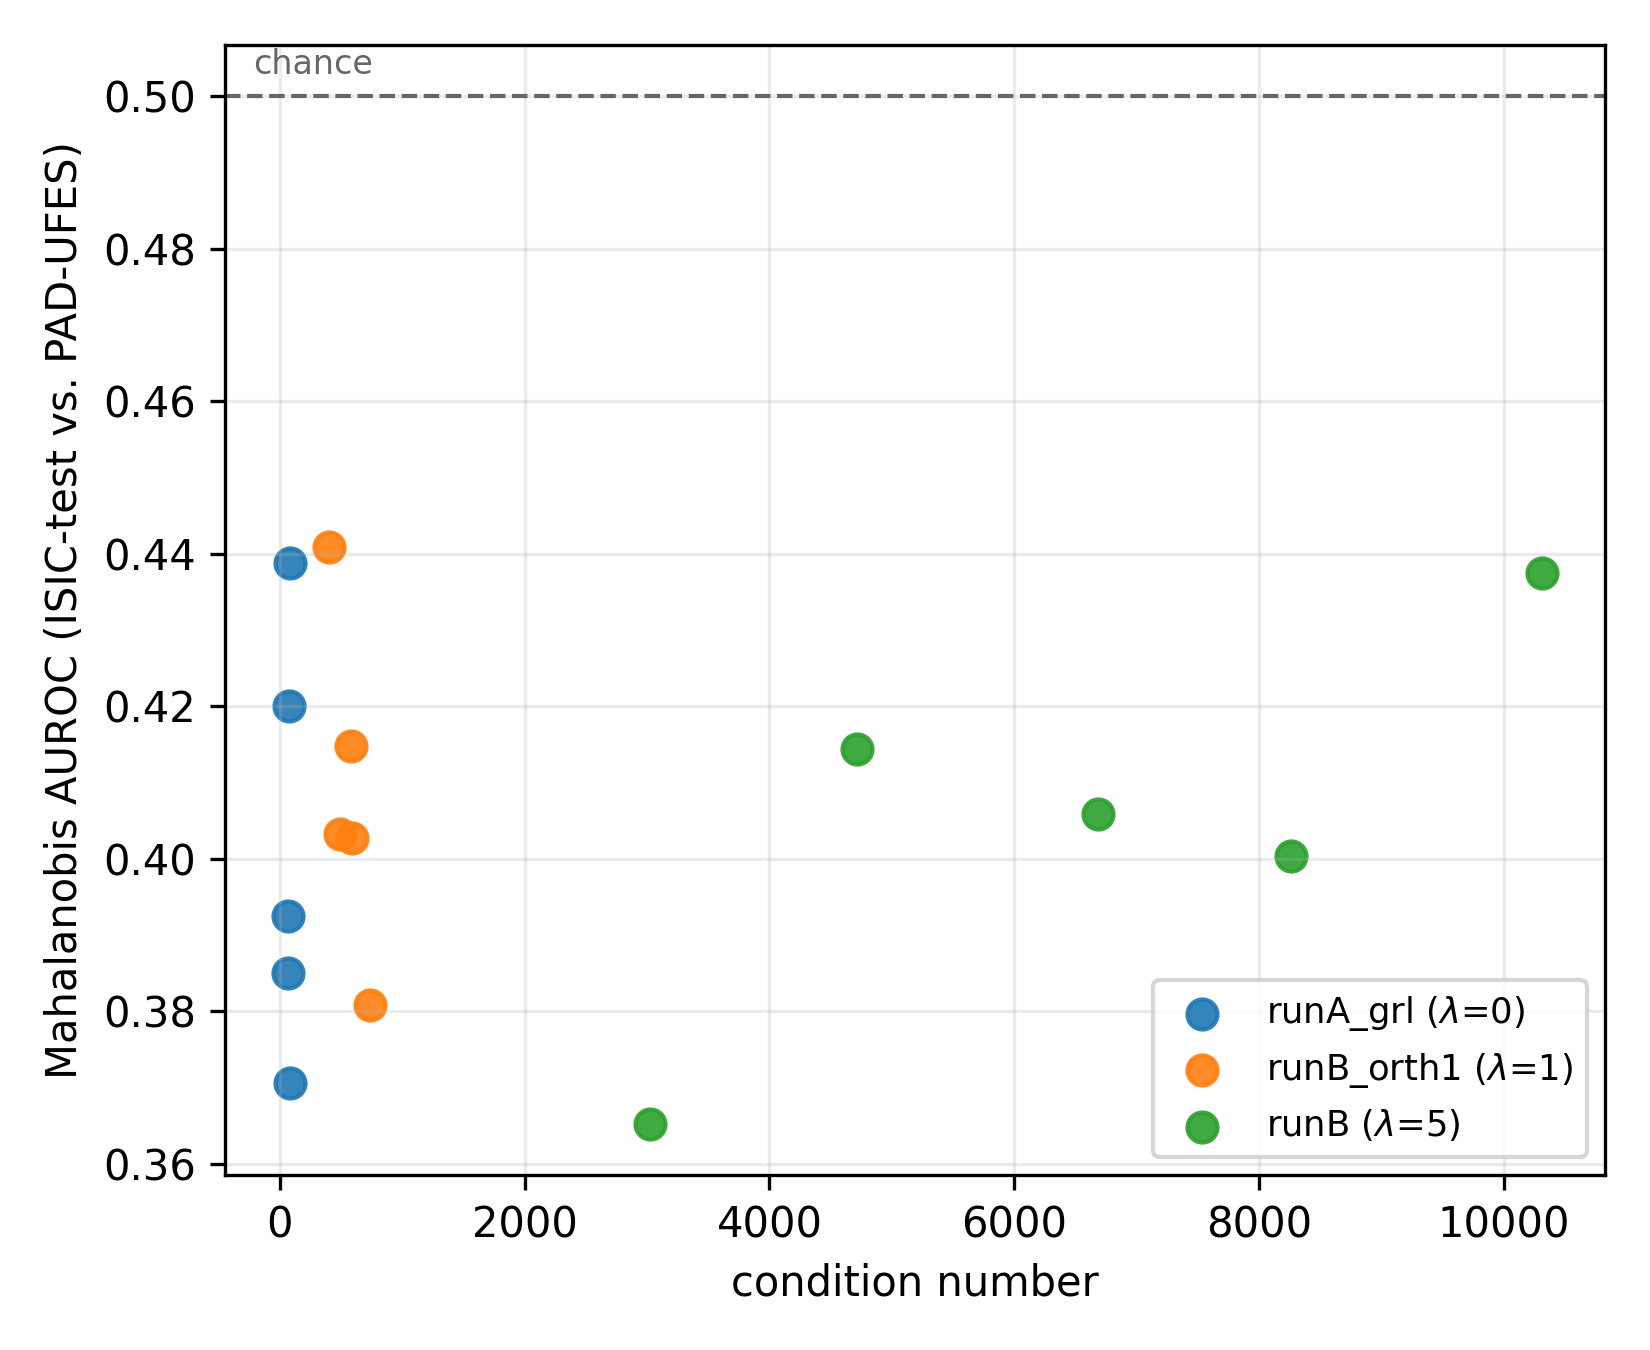
\includegraphics[width=0.6\linewidth]{figs/fig3_geometry_vs_auroc.png}
\caption{Representation geometry does not predict Mahalanobis AUROC. Condition number vs.\ Mahalanobis-distance AUROC (ISIC-test vs.\ PAD-UFES), one point per checkpoint, colored by rung. No association is apparent (Kendall's $\tau = -0.13$, $p = 0.59$; Table~\ref{tab:geometry}); the remaining four geometry metrics show the same pattern.}
\label{fig:geometry-vs-auroc}
\end{figure}
